\documentclass[]{article}
\usepackage{lmodern}
\usepackage{amssymb,amsmath}
\usepackage{ifxetex,ifluatex}
\usepackage{fixltx2e} % provides \textsubscript
\ifnum 0\ifxetex 1\fi\ifluatex 1\fi=0 % if pdftex
  \usepackage[T1]{fontenc}
  \usepackage[utf8]{inputenc}
\else % if luatex or xelatex
  \ifxetex
    \usepackage{mathspec}
  \else
    \usepackage{fontspec}
  \fi
  \defaultfontfeatures{Ligatures=TeX,Scale=MatchLowercase}
\fi
% use upquote if available, for straight quotes in verbatim environments
\IfFileExists{upquote.sty}{\usepackage{upquote}}{}
% use microtype if available
\IfFileExists{microtype.sty}{%
\usepackage{microtype}
\UseMicrotypeSet[protrusion]{basicmath} % disable protrusion for tt fonts
}{}
\usepackage[margin=1in]{geometry}
\usepackage{hyperref}
\hypersetup{unicode=true,
            pdftitle={Laborator 5},
            pdfborder={0 0 0},
            breaklinks=true}
\urlstyle{same}  % don't use monospace font for urls
\usepackage{color}
\usepackage{fancyvrb}
\newcommand{\VerbBar}{|}
\newcommand{\VERB}{\Verb[commandchars=\\\{\}]}
\DefineVerbatimEnvironment{Highlighting}{Verbatim}{commandchars=\\\{\}}
% Add ',fontsize=\small' for more characters per line
\usepackage{framed}
\definecolor{shadecolor}{RGB}{248,248,248}
\newenvironment{Shaded}{\begin{snugshade}}{\end{snugshade}}
\newcommand{\KeywordTok}[1]{\textcolor[rgb]{0.13,0.29,0.53}{\textbf{#1}}}
\newcommand{\DataTypeTok}[1]{\textcolor[rgb]{0.13,0.29,0.53}{#1}}
\newcommand{\DecValTok}[1]{\textcolor[rgb]{0.00,0.00,0.81}{#1}}
\newcommand{\BaseNTok}[1]{\textcolor[rgb]{0.00,0.00,0.81}{#1}}
\newcommand{\FloatTok}[1]{\textcolor[rgb]{0.00,0.00,0.81}{#1}}
\newcommand{\ConstantTok}[1]{\textcolor[rgb]{0.00,0.00,0.00}{#1}}
\newcommand{\CharTok}[1]{\textcolor[rgb]{0.31,0.60,0.02}{#1}}
\newcommand{\SpecialCharTok}[1]{\textcolor[rgb]{0.00,0.00,0.00}{#1}}
\newcommand{\StringTok}[1]{\textcolor[rgb]{0.31,0.60,0.02}{#1}}
\newcommand{\VerbatimStringTok}[1]{\textcolor[rgb]{0.31,0.60,0.02}{#1}}
\newcommand{\SpecialStringTok}[1]{\textcolor[rgb]{0.31,0.60,0.02}{#1}}
\newcommand{\ImportTok}[1]{#1}
\newcommand{\CommentTok}[1]{\textcolor[rgb]{0.56,0.35,0.01}{\textit{#1}}}
\newcommand{\DocumentationTok}[1]{\textcolor[rgb]{0.56,0.35,0.01}{\textbf{\textit{#1}}}}
\newcommand{\AnnotationTok}[1]{\textcolor[rgb]{0.56,0.35,0.01}{\textbf{\textit{#1}}}}
\newcommand{\CommentVarTok}[1]{\textcolor[rgb]{0.56,0.35,0.01}{\textbf{\textit{#1}}}}
\newcommand{\OtherTok}[1]{\textcolor[rgb]{0.56,0.35,0.01}{#1}}
\newcommand{\FunctionTok}[1]{\textcolor[rgb]{0.00,0.00,0.00}{#1}}
\newcommand{\VariableTok}[1]{\textcolor[rgb]{0.00,0.00,0.00}{#1}}
\newcommand{\ControlFlowTok}[1]{\textcolor[rgb]{0.13,0.29,0.53}{\textbf{#1}}}
\newcommand{\OperatorTok}[1]{\textcolor[rgb]{0.81,0.36,0.00}{\textbf{#1}}}
\newcommand{\BuiltInTok}[1]{#1}
\newcommand{\ExtensionTok}[1]{#1}
\newcommand{\PreprocessorTok}[1]{\textcolor[rgb]{0.56,0.35,0.01}{\textit{#1}}}
\newcommand{\AttributeTok}[1]{\textcolor[rgb]{0.77,0.63,0.00}{#1}}
\newcommand{\RegionMarkerTok}[1]{#1}
\newcommand{\InformationTok}[1]{\textcolor[rgb]{0.56,0.35,0.01}{\textbf{\textit{#1}}}}
\newcommand{\WarningTok}[1]{\textcolor[rgb]{0.56,0.35,0.01}{\textbf{\textit{#1}}}}
\newcommand{\AlertTok}[1]{\textcolor[rgb]{0.94,0.16,0.16}{#1}}
\newcommand{\ErrorTok}[1]{\textcolor[rgb]{0.64,0.00,0.00}{\textbf{#1}}}
\newcommand{\NormalTok}[1]{#1}
\usepackage{graphicx,grffile}
\makeatletter
\def\maxwidth{\ifdim\Gin@nat@width>\linewidth\linewidth\else\Gin@nat@width\fi}
\def\maxheight{\ifdim\Gin@nat@height>\textheight\textheight\else\Gin@nat@height\fi}
\makeatother
% Scale images if necessary, so that they will not overflow the page
% margins by default, and it is still possible to overwrite the defaults
% using explicit options in \includegraphics[width, height, ...]{}
\setkeys{Gin}{width=\maxwidth,height=\maxheight,keepaspectratio}
\IfFileExists{parskip.sty}{%
\usepackage{parskip}
}{% else
\setlength{\parindent}{0pt}
\setlength{\parskip}{6pt plus 2pt minus 1pt}
}
\setlength{\emergencystretch}{3em}  % prevent overfull lines
\providecommand{\tightlist}{%
  \setlength{\itemsep}{0pt}\setlength{\parskip}{0pt}}
\setcounter{secnumdepth}{5}
% Redefines (sub)paragraphs to behave more like sections
\ifx\paragraph\undefined\else
\let\oldparagraph\paragraph
\renewcommand{\paragraph}[1]{\oldparagraph{#1}\mbox{}}
\fi
\ifx\subparagraph\undefined\else
\let\oldsubparagraph\subparagraph
\renewcommand{\subparagraph}[1]{\oldsubparagraph{#1}\mbox{}}
\fi

%%% Use protect on footnotes to avoid problems with footnotes in titles
\let\rmarkdownfootnote\footnote%
\def\footnote{\protect\rmarkdownfootnote}

%%% Change title format to be more compact
\usepackage{titling}

% Create subtitle command for use in maketitle
\newcommand{\subtitle}[1]{
  \posttitle{
    \begin{center}\large#1\end{center}
    }
}

\setlength{\droptitle}{-2em}
  \title{Laborator 5}
  \pretitle{\vspace{\droptitle}\centering\huge}
  \posttitle{\par}
\subtitle{Compararea proporțiilor și tabele de contingență}
  \author{}
  \preauthor{}\postauthor{}
  \date{}
  \predate{}\postdate{}

\usepackage{booktabs}
\usepackage{longtable}
\usepackage{framed,color}
\definecolor{shadecolor}{RGB}{248, 248, 248}
%\definecolor{shadecolor1}{RGB}{216,225,235}
%\definecolor{framecolor}{RGB}{108,123,13}

%\definecolor{shadecolor}{RGB}{226, 255, 241}
\definecolor{shadecolor1}{RGB}{217,225,199}
\definecolor{framecolor}{RGB}{60,179,113}

\ifxetex
  \usepackage{letltxmacro}
  \setlength{\XeTeXLinkMargin}{1pt}
  \LetLtxMacro\SavedIncludeGraphics\includegraphics
  \def\includegraphics#1#{% #1 catches optional stuff (star/opt. arg.)
    \IncludeGraphicsAux{#1}%
  }%
  \newcommand*{\IncludeGraphicsAux}[2]{%
    \XeTeXLinkBox{%
      \SavedIncludeGraphics#1{#2}%
    }%
  }%
\fi

\newenvironment{frshaded*}{%
  \def\FrameCommand{\fboxrule=\FrameRule\fboxsep=\FrameSep \fcolorbox{framecolor}{shadecolor1}}%
  \MakeFramed {\advance\hsize-\width \FrameRestore}}%
{\endMakeFramed}

\newenvironment{rmdblock}[1]
  {\begin{frshaded*}
  \begin{itemize}
  \renewcommand{\labelitemi}{
    \raisebox{-.7\height}[0pt][0pt]{
      {\setkeys{Gin}{width=2em,keepaspectratio}\includegraphics{images/icons/#1}}
    }
  }
  \item
  }
  {
  \end{itemize}
  \end{frshaded*}
  }

\newenvironment{rmdcaution}
  {\begin{rmdblock}{caution}}
  {\end{rmdblock}}
% \newenvironment{rmdinsight}
%   {\begin{rmdblock}{insight}}
%   {\end{rmdblock}}
\newenvironment{rmdexercise}
  {\begin{rmdblock}{exercise}}
  {\end{rmdblock}}
\newenvironment{rmdtip}
  {\begin{rmdblock}{tip}}
  {\end{rmdblock}}


%%%%%%%%%%%%%%%%%%%%%%%%%%%%%%%%%%%%%%%%%%%%%%%%%%%%%%%%%%%%%%%%%%%%%%%%%%%%%%%%%%%%%%%%%%%%%%%%%%%%%%%%%%%%%%%%%%%%%
%%%%%%%%%%% For insight block %%%%%%%%%%%%%%%%%%%%%%%%%%
\definecolor{shadecolor_insight}{RGB}{223,240,216}
\definecolor{framecolor_insight}{RGB}{136,193,137}

%\definecolor{shadecolor_insight}{RGB}{217,225,199}
%\definecolor{framecolor_insight}{RGB}{60,179,113}

\newenvironment{frshaded_insight*}{%
  \def\FrameCommand{\fboxrule=\FrameRule\fboxsep=\FrameSep \fcolorbox{framecolor_insight}{shadecolor_insight}}%
  \MakeFramed {\advance\hsize-\width \FrameRestore}}%
{\endMakeFramed}

\newenvironment{rmdblock_insight}[1]
  {\begin{frshaded_insight*}
  \begin{itemize}
  \renewcommand{\labelitemi}{
    \raisebox{-.7\height}[0pt][0pt]{
      {\setkeys{Gin}{width=2em,keepaspectratio}\includegraphics{images/icons/#1}}
    }
  }
  \item
  }
  {
  \end{itemize}
  \end{frshaded_insight*}
  }

\newenvironment{rmdinsight}
  {\begin{rmdblock_insight}{insight}}
  {\end{rmdblock_insight}}

%%%%%%%%%%%%%%%%%%%%%%%%%%%%%%%%%%%%%%%%%%%%%%%%%%%%%%%%%%%%%%%%%%%%%%%%%%%%%%%%%%%%%%%%%%%%%%%%%%%%%%%%%%%%%%%%%%%%%
\usepackage{subfigure}
\usepackage{booktabs}
\usepackage{slashbox}
\usepackage{color}
%%%%%%%%%%%%%%%%%%%%%%%%%%%%%%%%%%%%%%%%%%%%%%%%%%%%%%%%%%%%%%%%%%%%%%%%%%%%%%%%%%%%%%%%%%%%%%%%%%%%%%%%%%%%%%%%%%%%%
%CITEVA DEFINITII
\def\om{\omega}
\def\Om{\Omega}
\def\et{\eta}
\def\td{\tilde{\delta}}
\def\m{{\mu}}
\def\n{{\nu}}
\def\k{{\kappa}}
\def\l{{\lambda}}
\def\L{{\Lambda}}
\def\g{{\gamma}}
\def\a{{\alpha}}
\def\e{{\varepsilon}}
\def\b{{\beta}}
\def\G{{\Gamma}}
\def\d{{\delta}}
\def\D{{\Delta}}
\def\t{{\theta}}
\def\s{{\sigma}}
\def\S{{\Sigma}}
\def\z{{\zeta}}
\def\qed{\hfill\Box}
\def\ds{\displaystyle}
\def\mc{\mathcal}
%%%%%%%%%%%%%%%%%%%%%%%%%%%%%%%%%%%%%%%%%%%%%%%%%%%%%%%%%%%%%%%%%%%%%%%%%%%%%%%%%%%%%%%%%%%%%%%%%%%%%%%%%%%%%%%%%%%%%%
\def\1{{\mathbf 1}}
\def\CC{{\mathbb C}}
\def\VV{{\mathbb V}}
\def\RR{{\mathbb R}}
\def\QQ{{\mathbb Q}}
\def\ZZ{{\mathbb Z}}
\def\PP{{\mathbb P}}
\def\EE{{\mathbb E}}
\def\NN{{\mathbb N}}
\def\FF{{\mathbb F}}
%\def\SS{{\mathbb S}}
\def\MA{{\mathcal A}}
\def\MO{{\mathcal O}}
\def\MF{{\mathcal F}}
\def\ME{{\mathcal E}}
\def\MR{{\mathcal R}}
\def\MB{{\mathcal B}}
\def\MM{{\mathcal M}}
\def\MN{{\mathcal N}}
\def\MU{{\mathcal U}}
\def\MP{{\mathcal P}}
\def\MS{{\mathcal S}}
\def\MBS{{\mathbf S}}
\def\MX{{\bm{ \mathscr X}}}

% independent sign
\newcommand\independent{\protect\mathpalette{\protect\independenT}{\perp}}
\def\independenT#1#2{\mathrel{\rlap{$#1#2$}\mkern2mu{#1#2}}}

\renewcommand\tablename{Tab.}
\renewcommand{\figurename}{Fig.}
\renewcommand\refname{Referințe}

%%%%%%%%%%%%%%%%%%%%%%%%%%%%%%%%%%%%%%%%%%%%%%%%%%%%%%%%%%%%%%%%%%%%%%%%%%%%%%%%%%%%%%%%%%%%%%%%%%%%%%%%%%%%%%%%%%%%%
%Header and Footer
\usepackage{fancyhdr}

\pagestyle{fancy}
\fancyhf{}
\rhead{Universitatea din Bucure\c sti\\ Facultatea de Matematic\u a \c si Informatic\u a}
\lhead{\textit{Curs}: Biostatistic\u a 2018\\ \textit{Instructor}: A. Am\u arioarei}
\rfoot{Pagina \thepage}
\lfoot{Grupa: 503}
%%%%%%%%%%%%%%%%%%%%%%%%%%%%%%%%%%%%%%%
\usepackage{booktabs}
\usepackage{longtable}
\usepackage{array}
\usepackage{multirow}
\usepackage[table]{xcolor}
\usepackage{wrapfig}
\usepackage{float}
\usepackage{colortbl}
\usepackage{pdflscape}
\usepackage{tabu}
\usepackage{threeparttable}
\usepackage{threeparttablex}
\usepackage[normalem]{ulem}
\usepackage{makecell}

\begin{document}
\maketitle

%%%%%%%%%%%%%%%%%%%%%%%%
\thispagestyle{fancy}

Obiectivul acestui laborator este de a prezenta câteva teste statistice
folosite pentru testarea ipotezelor statistice atunci când datele sunt
de tip categoric.

\section{\texorpdfstring{Compararea proporțiilor și tabele de
contingență
\(2\times 2\)}{Compararea proporțiilor și tabele de contingență 2\textbackslash{}times 2}}\label{compararea-proportiilor-si-tabele-de-contingenta-2times-2}

Considerăm următorul exemplu:

\begin{rmdexercise}
Un studiu clinic a investigat efectele metodelor contraceptive orale
(OC) asupra bolilor de inimă la femeile cu vârste între 40 și 44 de ani.
Cercetătorii au găsit că printre 5000 de femei care utilizau metode
contraceptive orale la momentul studiului (cazuri), 13 dintre acestea au
dezvoltat un infarct miocardic (MI) (pe o perioadă de 3 ani) pe când
printre 10000 de femei care nu au folosit niciodată OC (grupul de
control) doar 7 au dezvoltat MI (pe aceeași perioadă). Vrem să vedem
dacă există vreo asociere între consumul de anticoncepționale pe cale
orală și incidența infarctului miocardic (pe această perioadă).
\end{rmdexercise}

Fie \(\pi_1=\mathbb{P}(MI\,|\,OC)\), probabilitatea ca femeile să
dezvolte infarct miocardic (MI) în cazul grupului care a consumat
contraceptive orale (OC) și \(\pi_2=\mathbb{P}(MI\,|\,non-OC)\),
probabilitatea ca femeile să dezvolte infarct miocardic (MI) în cazul
grupului care nu a consumat contraceptive orale (OC). Întrebarea este
dacă probabilitatea de a face infarct miocardic diferă între cele două
grupuri (cazuri vs control). Cu alte cuvinte vrem să testăm ipotezele
statistice:

\[
  \begin{array}{ll}
    H_0:\,\,\pi_1=\pi_2\\
    H_1:\,\,\pi_1\neq \pi_2
  \end{array}
\]

\subsection{Compararea proporțiilor prin aproximarea
normală}\label{compararea-proportiilor-prin-aproximarea-normala}

Putem modela problema astfel: considerăm
\(X_1, X_2, \ldots, X_{n_1}\in\{0,1\}\) (\(0\) - nu a dezvoltat infarct
miocardic, \(1\) - a dezvoltat infarct miocardic pe perioada studiului)
un eșantion de talie \(n_1\) (\(n_1 = 5000\)) dintr-o populație
Bernoulli \(\mathcal{B}(\pi_1)\) care să reprezinte populația femeilor
cu vârste între 40 și 44 de ani care au consumat contraceptive orale
(cazuri) și respectiv un eșantion
\(Y_1, Y_2, \ldots, Y_{n_2}\in\{0,1\}\) un eșantion de talie \(n_2\)
(\(n_2 = 10000\)) dintr-o populație Bernoulli \(\mathcal{B}(\pi_2)\)
care să reprezinte populația femeilor cu vârste între 40 și 44 de ani
care nu au consumat contraceptive orale (control). Vom presupune că
eșantioanele sunt suficient de mari pentru a putea aplica aproximarea
normală a binomialei (e.g.~vezi
\href{https://alexamarioarei.github.io/Teaching/2017-2018/PS\%20web\%20page/labs/Lab_4.html\#3_aproximarea_poisson_\%C8\%99i_normal\%C4\%83_a_binomialei}{aici}).

Se poate verifica cu ușurință că sub \(H_0:\,\pi_1=\pi_2=\pi\) are loc

\[
  \hat{\pi}_1 - \hat{\pi}_2\sim\mathcal{N}\left(\underbrace{\pi_1-\pi_2}_{=0}, \pi(1-\pi)\left(\frac{1}{n_1} + \frac{1}{n_2}\right)\right)
\]

unde \(\hat{\pi}_1 = \bar{X}_{n_1}\) iar
\(\hat{\pi}_2 = \bar{Y}_{n_2}\). Astfel, sub \(H_0\), avem

\[
  Z = \frac{\hat{\pi}_1 - \hat{\pi}_2}{\sqrt{\pi(1-\pi)\left(\frac{1}{n_1} + \frac{1}{n_2}\right)}} \sim \mathcal{N}(0,1)
\]

și cum \(\pi\) este necunoscut putem să-l aproximăm din cele două
eșantioane luate împreună (estimatorul \emph{pooled})

\[
  \hat{\pi} = \frac{\sum_{i = 1}^{n_1}X_i + \sum_{j = 1}^{n_2}Y_j}{n_1+n_2} = \frac{n_1\hat{\pi}_1 + n_2\hat{\pi}_2}{n_1+n_2}.
\]

Dacă luăm în calcul corecția de continuitate a aproximării normale a
binomialei atunci regiunea critică a testului bilateral de nivel
\(\alpha\) (acest test se numește \emph{testul de scor} și este
recomandat atunci când vrem să comparîăm proporții în locul
\emph{testului lui Wald}), cu ipotezele statistice
\(H_0:\,\pi_1=\pi_2\,\,vs\,\,H_1:\,\pi_1\neq \pi_2\), este

\[
  C = \left\{(x_1,\ldots,x_{n_1},y_1,\ldots,y_{n_2})\,|\,\frac{|\hat{\pi}_1 - \hat{\pi}_2| - \frac{1}{2}\left(\frac{1}{n_1} + \frac{1}{n_2}\right)}{\sqrt{\hat{\pi}(1-\hat{\pi})\left(\frac{1}{n_1} + \frac{1}{n_2}\right)}}>z_{1-\frac{\alpha}{2}}\right\}
\]

iar p-valoarea aproximativă a testului este

\[
  p-val = 2(1-\Phi(z_{\text{obs}})).
\]

De regulă, în practică, putem folosi aproximarea normală a binomialei și
testul de comparare a proporțiilor cu regiunea critică \(C\) atunci când
sunt îndeplinite condițiile \(n_1\hat{\pi}(1-\hat{\pi})\geq 5\) și
\(n_2\hat{\pi}(1-\hat{\pi})\geq 5\).

În R avem

\begin{Shaded}
\begin{Highlighting}[]
\NormalTok{n1 =}\StringTok{ }\DecValTok{5000} \CommentTok{# nr total cazuri OC}
\NormalTok{n11 =}\StringTok{ }\DecValTok{13} \CommentTok{# nr cazuri cu MI}

\NormalTok{n2 =}\StringTok{ }\DecValTok{10000} \CommentTok{# nr total control non-OC}
\NormalTok{n21 =}\StringTok{ }\DecValTok{7} \CommentTok{# nr control cu MI}

\NormalTok{p1 =}\StringTok{ }\NormalTok{n11}\OperatorTok{/}\NormalTok{n1}
\NormalTok{p2 =}\StringTok{ }\NormalTok{n21}\OperatorTok{/}\NormalTok{n2}

\NormalTok{p =}\StringTok{ }\NormalTok{(n11}\OperatorTok{+}\NormalTok{n21)}\OperatorTok{/}\NormalTok{(n1}\OperatorTok{+}\NormalTok{n2) }\CommentTok{# proportia comuna - pooled p}
\end{Highlighting}
\end{Shaded}

și putem verifica cele două condiții de aplicabilitate a aproximării
normale

\begin{Shaded}
\begin{Highlighting}[]
\CommentTok{# Verificam daca putem aplica aproximarea normala }
\NormalTok{n1}\OperatorTok{*}\NormalTok{p}\OperatorTok{*}\NormalTok{(}\DecValTok{1}\OperatorTok{-}\NormalTok{p)}\OperatorTok{>}\DecValTok{5}
\NormalTok{[}\DecValTok{1}\NormalTok{] }\OtherTok{TRUE}
\NormalTok{n2}\OperatorTok{*}\NormalTok{p}\OperatorTok{*}\NormalTok{(}\DecValTok{1}\OperatorTok{-}\NormalTok{p)}\OperatorTok{>}\DecValTok{5}
\NormalTok{[}\DecValTok{1}\NormalTok{] }\OtherTok{TRUE}
\end{Highlighting}
\end{Shaded}

Calculul statisticii de test și a p-valorii testului, pentru exemplul
nostru, sunt

\begin{Shaded}
\begin{Highlighting}[]
\CommentTok{# Calculam statistica de test cu corectia de continuitate}
\NormalTok{z =}\StringTok{ }\NormalTok{(}\KeywordTok{abs}\NormalTok{(p1}\OperatorTok{-}\NormalTok{p2)}\OperatorTok{-}\FloatTok{0.5}\OperatorTok{*}\NormalTok{(}\DecValTok{1}\OperatorTok{/}\NormalTok{n1}\OperatorTok{+}\DecValTok{1}\OperatorTok{/}\NormalTok{n2))}\OperatorTok{/}\KeywordTok{sqrt}\NormalTok{(p}\OperatorTok{*}\NormalTok{(}\DecValTok{1}\OperatorTok{-}\NormalTok{p)}\OperatorTok{*}\NormalTok{(}\DecValTok{1}\OperatorTok{/}\NormalTok{n1}\OperatorTok{+}\DecValTok{1}\OperatorTok{/}\NormalTok{n2))}
\NormalTok{z}
\NormalTok{[}\DecValTok{1}\NormalTok{] }\FloatTok{2.768839}

\CommentTok{# Calcul de p-valoare: test bilateral}
\NormalTok{pval =}\StringTok{ }\KeywordTok{min}\NormalTok{(}\DecValTok{2}\OperatorTok{*}\NormalTok{(}\DecValTok{1}\OperatorTok{-}\KeywordTok{pnorm}\NormalTok{(z)), }\DecValTok{1}\NormalTok{)}
\NormalTok{pval}
\NormalTok{[}\DecValTok{1}\NormalTok{] }\FloatTok{0.005625635}
\end{Highlighting}
\end{Shaded}

Observăm că același răspuns se obține și dacă folosim funcția
\texttt{prop.test()} din R:

\begin{Shaded}
\begin{Highlighting}[]
\KeywordTok{prop.test}\NormalTok{(}\KeywordTok{c}\NormalTok{(}\DecValTok{13}\NormalTok{, }\DecValTok{7}\NormalTok{), }\KeywordTok{c}\NormalTok{(}\DecValTok{5000}\NormalTok{, }\DecValTok{10000}\NormalTok{))}

    \DecValTok{2}\OperatorTok{-}\NormalTok{sample test }\ControlFlowTok{for}\NormalTok{ equality of proportions with continuity}
\NormalTok{    correction}

\NormalTok{data}\OperatorTok{:}\StringTok{  }\KeywordTok{c}\NormalTok{(}\DecValTok{13}\NormalTok{, }\DecValTok{7}\NormalTok{) out of }\KeywordTok{c}\NormalTok{(}\DecValTok{5000}\NormalTok{, }\DecValTok{10000}\NormalTok{)}
\NormalTok{X}\OperatorTok{-}\NormalTok{squared =}\StringTok{ }\FloatTok{7.6665}\NormalTok{, df =}\StringTok{ }\DecValTok{1}\NormalTok{, p}\OperatorTok{-}\NormalTok{value =}\StringTok{ }\FloatTok{0.005626}
\NormalTok{alternative hypothesis}\OperatorTok{:}\StringTok{ }\NormalTok{two.sided}
\DecValTok{95}\NormalTok{ percent confidence interval}\OperatorTok{:}
\StringTok{ }\FloatTok{0.0002463116} \FloatTok{0.0035536884}
\NormalTok{sample estimates}\OperatorTok{:}
\NormalTok{prop }\DecValTok{1}\NormalTok{ prop }\DecValTok{2} 
\FloatTok{0.0026} \FloatTok{0.0007} 
\end{Highlighting}
\end{Shaded}

De asemenea putem construi și intervalul de încredere de nivel
\(1-\alpha\), corespunzător

\begin{verbatim}
IC pentru pi1-pi2 la pragul de semnificatie 95% este 
 IC = [ 0.0006612366 , 0.003138763 ]
\end{verbatim}

precum și intervalul de încredere clasic pentru diferența proporțiilor,
obținut prin aproximarea lui Wald

\[
  \hat{\pi}_1 - \hat{\pi}_2 \pm z_{1-\frac{\alpha}{2}}\sqrt{\frac{\hat{\pi}_1(1-\hat{\pi}_1)}{n_1} + \frac{\hat{\pi}_2(1-\hat{\pi}_2)}{n_2}}
\]

\begin{verbatim}
IC pentru pi1-pi2 la pragul de semnificatie 95% este 
 IC = [ 0.0003963116 , 0.003403688 ]
\end{verbatim}

În articolul (Agresti 2000), autorii prezintă un alt interval de
încredere (ajustat prin adăugarea a două observații la fiecare eșantion,
un \(1\) și un \(0\)) pentru diferența proporțiilor

\[
  \bar{\pi}_1 - \bar{\pi}_2 \pm z_{1-\frac{\alpha}{2}}\sqrt{\frac{\bar{\pi}_1(1-\bar{\pi}_1)}{n_1+2} + \frac{\bar{\pi}_2(1-\bar{\pi}_2)}{n_2+2}}
\]

unde \(\bar{\pi}_1 = \frac{\sum_{i = 1}^{n_1}X_i + 1}{n_1+2}\) iar
\(\bar{\pi}_2 = \frac{\sum_{j = 1}^{n_1}Y_j + 1}{n_2+2}\)

\begin{verbatim}
IC (Agresti-Caffo) pentru pi1-pi2 la pragul de semnificatie 95% este 
 IC = [ 0.0006853283 , 0.003312753 ]
\end{verbatim}

\begin{center}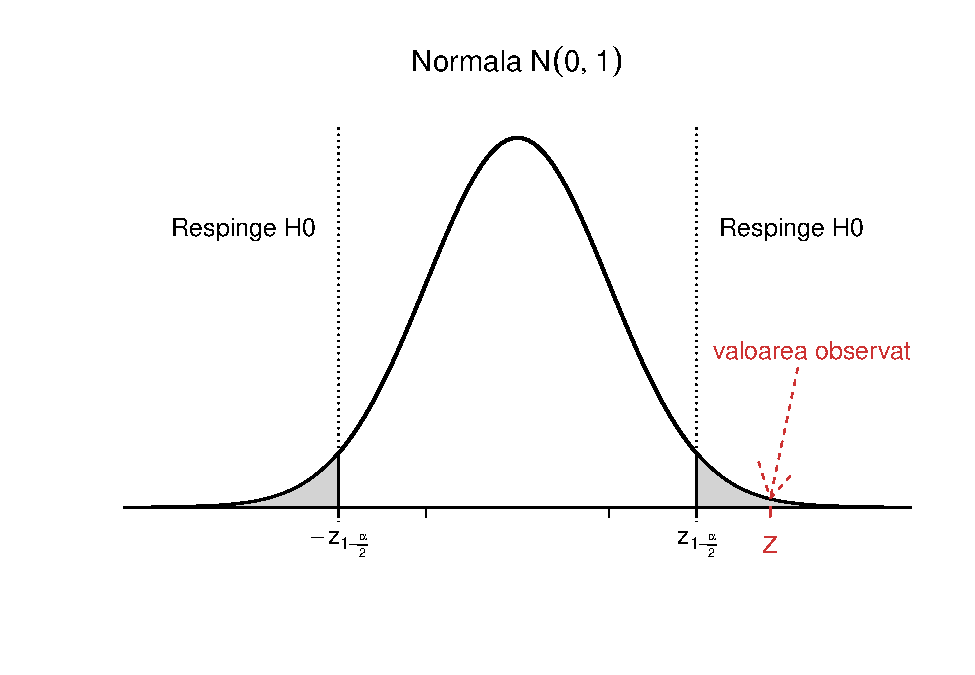
\includegraphics[width=0.8\linewidth]{Lab_5_files/figure-latex/unnamed-chunk-10-1} \end{center}

Concluzionăm că folosirea de anticoncepționale pe cale orală este
semnificativ asociată cu incidența crescută de cazuri de MI la femeile
cu vârste între 40 și 44 de ani pe perioada de 3 ani a studiului.

\begin{rmdexercise}
Puteți crea o funcție care să automatizeze procesul ?
\end{rmdexercise}

\subsection{\texorpdfstring{Metoda tabelelor de contingență și testul
\(\chi^2\) al lui
Pearson}{Metoda tabelelor de contingență și testul \textbackslash{}chi\^{}2 al lui Pearson}}\label{metoda-tabelelor-de-contingenta-si-testul-chi2-al-lui-pearson}

Rescriem problema de mai sus sub formă de tabel de contingență
\(2\times2\) (un tabel în care datele apar clasificate după valorile a
două variabile categorice, cu două clase fiecare) pentru vectorul
aleator
\((X,Y)\in\{a_1, a_2\}\times\{b_1,b_2\} = \{\text{OC}, \text{non-OC}\}\times\{\text{MI},\text{non-MI}\}\):

\[
  \begin{array}{c|c|c|c}
    X/Y & b_1 & b_2 & \text{Total}\\
    \hline
    a_1 & n_{11} & n_{12} & n_{1\cdot} = n_{11} + n_{12}\\
    \hline
    a_2 & n_{21} & n_{22} & n_{2\cdot} = n_{21} + n_{22}\\
    \hline
    \text{Total} & n_{\cdot 1} = n_{11} + n_{21} & n_{\cdot 2} = n_{12} + n_{22} & n = \sum_{i,j = 1}^{2}n_{ij}\\
  \end{array}
\] care în cazul problemei noastre este

\rowcolors{2}{gray!6}{white}

\begin{longtable}{lccccccccc}
\hiderowcolors
\toprule
  & MI & non-MI & Total\\
\midrule
\endfirsthead
\multicolumn{10}{@{}l}{\textit{(continued)}}\\
\toprule
  & MI & non-MI & Total\\
\midrule
\endhead
\
\endfoot
\bottomrule
\endlastfoot
\showrowcolors
OC & 13 & 4987 & 5000\\
non-OC & 7 & 9993 & 10000\\
Total & 20 & 14980 & 15000\\*
\end{longtable}

\rowcolors{2}{white}{white}

Acesta se mai numește și tabelul observat

\[
  \text{Tabel}_{obs} = \begin{array}{c|c}
      O_{11} & O_{12}\\
      \hline
      O_{21} & O_{22}
  \end{array} = \begin{array}{c|c}
      n_{11} & n_{12}\\
      \hline
      n_{21} & n_{22}
  \end{array}
\] Repartiția vectorului \((X,Y)\) este dată de
\(\mathbb{P}\circ (X,Y)^{-1} = \sum_{i = 1}^{2}\sum_{j = 1}^{2}p_{ij}\delta_{(a_i,b_j)}\),
unde \(\mathbb{P}((X,Y) = (a_i, b_j)) = p_{ij}\)

\[
  \begin{array}{c|c|c|c}
    X/Y & b_1 & b_2 & \sum\\
    \hline
    a_1 & p_{11} & p_{12} & p_1 = p_{11} + p_{12}\\
    \hline
    a_2 & p_{21} & p_{22} & p_2 = p_{21} + p_{22}\\
    \hline
    \sum & q_1 = p_{11} + p_{21} & q_2 = p_{12} + p_{22} & 1\\
  \end{array}
\]

iar repartițiile marginale sunt
\(\mathbb{P}\circ X^{-1} = \sum_{i = 1}^{2}p_{i}\delta_{a_i}\),
\(\mathbb{P}\circ Y^{-1} = \sum_{j = 1}^{2}q_{j}\delta_{b_j}\) cu
\(\mathbb{P}(X = a_i) = p_i\) și respectiv
\(\mathbb{P}(Y = b_j) = q_j\).

Suntem interesați în testarea ipotezelor

\[
H_0:\, \pi_1 = \pi_2\,\, vs \,\, H_1:\,\pi_1 \neq \pi_2
\]

unde \(\pi_1=\mathbb{P}(MI\,|\,OC) = \mathbb{P}(Y = b_1\,|\,X = a_1)\)
iar
\(\pi_2=\mathbb{P}(MI\,|\,non-OC) = \mathbb{P}(Y = b_1\,|\,X = a_2)\).
Observăm că

\[
  \pi_1 = \pi_2 \iff \frac{p_{11}}{p_1} = \frac{p_{21}}{p_2} \iff \frac{p_{11}}{p_1} = \frac{q_1 - p_{11}}{p_2} \iff p_{11} = p_1q_1
\] și, în mod similar, se poate verifica că \(p_{ij} = p_iq_j\),
\(\forall i,j\in\{1,2\}\). Cu alte cuvinte, ipoteza nulă se mai scrie și
sub forma

\[
  H_0:\, \{\pi_1 = \pi_2\} = \left\{p_{ij} = p_iq_j,\,\forall i,j\in\{1,2\}\right\}
\] Fie \((X_1, Y_1), (X_2, Y_2),\ldots,(X_n, Y_n)\) un eșantion de talie
\(n\) din populația \(\mathbb{P}\circ (X,Y)^{-1}\) și avem că
\(n_{ij} = \sum_{k = 1}^n\mathbf{1}_{(a_i, b_j)}(X_k, Y_k)\) (numărul de
observații din celula \((i,j)\)) iar
\(n_{i\cdot} = \sum_{j = 1}^{2}n_{ij}\),
\(n_{\cdot j} = \sum_{i = 1}^{2}n_{ij}\) și respectiv
\(n = \sum_{i,j = 1}^{2}n_{ij}\).

Sub ipoteza nulă, \(H_0\), avem că estimatorii de verosimilitate maximă
pentru \(p_i\) și \(q_j\) sunt

\[
  \hat{p}_i = \frac{n_{i\cdot}}{n},\,\, \hat{q}_j = \frac{n_{\cdot j}}{n}
\]

iar numărul de observații pe care ne așteptăm să-l observăm (sub
\(H_0\)) în fiecare celulă este

\[
  E_{ij} = n \hat{p}_{ij} \overset{H_0}{=} n \hat{p}_i \hat{q}_j = \frac{n_{i\cdot}n_{\cdot j}}{n}.
\] Astfel tabelul pe care ne așteptăm să-l observăm sub ipoteza nulă
este

\[
  \text{Tabel}_{exp} = \begin{array}{c|c}
      E_{11} & E_{12}\\
      \hline
      E_{21} & E_{22}
  \end{array} = \begin{array}{c|c}
      \frac{n_{1\cdot}n_{\cdot 1}}{n} & \frac{n_{1\cdot}n_{\cdot 2}}{n}\\
      \hline
      \frac{n_{2\cdot}n_{\cdot 1}}{n} & \frac{n_{2\cdot}n_{\cdot 2}}{n}
  \end{array}
\]

Calculul tabelului pe care ne așteptăm să-l observăm:

\begin{Shaded}
\begin{Highlighting}[]
\CommentTok{# Observat}
\NormalTok{n11 =}\StringTok{ }\DecValTok{13}
\NormalTok{n1o =}\StringTok{ }\DecValTok{5000}
\NormalTok{n12 =}\StringTok{ }\NormalTok{n1o}\OperatorTok{-}\NormalTok{n11}

\NormalTok{n21 =}\StringTok{ }\DecValTok{7}
\NormalTok{n2o =}\StringTok{ }\DecValTok{10000}
\NormalTok{n22 =}\StringTok{ }\NormalTok{n2o}\OperatorTok{-}\NormalTok{n21}

\NormalTok{no1 =}\StringTok{ }\NormalTok{n11}\OperatorTok{+}\NormalTok{n21}
\NormalTok{no2 =}\StringTok{ }\NormalTok{n12}\OperatorTok{+}\NormalTok{n22}

\NormalTok{n =}\StringTok{ }\NormalTok{n1o}\OperatorTok{+}\NormalTok{n2o}

\CommentTok{#Asteptat}
\NormalTok{e11 =}\StringTok{ }\NormalTok{n1o}\OperatorTok{*}\NormalTok{no1}\OperatorTok{/}\NormalTok{n}
\NormalTok{e12 =}\StringTok{ }\NormalTok{n1o}\OperatorTok{*}\NormalTok{no2}\OperatorTok{/}\NormalTok{n}
\NormalTok{e21 =}\StringTok{ }\NormalTok{n2o}\OperatorTok{*}\NormalTok{no1}\OperatorTok{/}\NormalTok{n}
\NormalTok{e22 =}\StringTok{ }\NormalTok{n2o}\OperatorTok{*}\NormalTok{no2}\OperatorTok{/}\NormalTok{n}

\NormalTok{Mobs =}\StringTok{ }\KeywordTok{matrix}\NormalTok{(}\KeywordTok{c}\NormalTok{(n11,n12,n21,n22),}\DataTypeTok{ncol =} \DecValTok{2}\NormalTok{, }\DataTypeTok{byrow =}\NormalTok{ T, }
              \DataTypeTok{dimnames =} \KeywordTok{list}\NormalTok{(}\KeywordTok{c}\NormalTok{(}\StringTok{"OC"}\NormalTok{,}\StringTok{"non-OC"}\NormalTok{), }\KeywordTok{c}\NormalTok{(}\StringTok{"MI"}\NormalTok{, }\StringTok{"non-MI"}\NormalTok{)))}

\NormalTok{Mexp =}\StringTok{ }\KeywordTok{matrix}\NormalTok{(}\KeywordTok{c}\NormalTok{(e11,e12,e21,e22),}\DataTypeTok{ncol =} \DecValTok{2}\NormalTok{, }\DataTypeTok{byrow =}\NormalTok{ T, }
              \DataTypeTok{dimnames =} \KeywordTok{list}\NormalTok{(}\KeywordTok{c}\NormalTok{(}\StringTok{"OC"}\NormalTok{,}\StringTok{"non-OC"}\NormalTok{), }\KeywordTok{c}\NormalTok{(}\StringTok{"MI"}\NormalTok{, }\StringTok{"non-MI"}\NormalTok{)))}
\end{Highlighting}
\end{Shaded}

\rowcolors{2}{gray!6}{white}

\begin{longtable}{lcccccc}
\hiderowcolors
\toprule
  & MI & non-MI\\
\midrule
\endfirsthead
\multicolumn{7}{@{}l}{\textit{(continued)}}\\
\toprule
  & MI & non-MI\\
\midrule
\endhead
\
\endfoot
\bottomrule
\endlastfoot
\showrowcolors
OC & 6.666667 & 4993.333\\
non-OC & 13.333333 & 9986.667\\*
\end{longtable}

\rowcolors{2}{white}{white}

Calculul statisticii de test cu corecția lui Yates:

\[
  X^2 = \sum_{i=1}^{2}\sum_{j=1}^{2}\frac{\left(|O_{ij}-E_{ij}|-0.5\right)^2}{E_{ij}}\underset{H_0}{\sim}\chi_1^2
\]

\begin{Shaded}
\begin{Highlighting}[]
\NormalTok{X2 =}\StringTok{ }\NormalTok{(}\KeywordTok{abs}\NormalTok{(n11}\OperatorTok{-}\NormalTok{e11)}\OperatorTok{-}\FloatTok{0.5}\NormalTok{)}\OperatorTok{^}\DecValTok{2}\OperatorTok{/}\NormalTok{e11 }\OperatorTok{+}\StringTok{ }\NormalTok{(}\KeywordTok{abs}\NormalTok{(n12}\OperatorTok{-}\NormalTok{e12)}\OperatorTok{-}\FloatTok{0.5}\NormalTok{)}\OperatorTok{^}\DecValTok{2}\OperatorTok{/}\NormalTok{e12 }\OperatorTok{+}\StringTok{ }
\StringTok{  }\NormalTok{(}\KeywordTok{abs}\NormalTok{(n21}\OperatorTok{-}\NormalTok{e21)}\OperatorTok{-}\FloatTok{0.5}\NormalTok{)}\OperatorTok{^}\DecValTok{2}\OperatorTok{/}\NormalTok{e21 }\OperatorTok{+}\StringTok{ }\NormalTok{(}\KeywordTok{abs}\NormalTok{(n22}\OperatorTok{-}\NormalTok{e22)}\OperatorTok{-}\FloatTok{0.5}\NormalTok{)}\OperatorTok{^}\DecValTok{2}\OperatorTok{/}\NormalTok{e22}
\NormalTok{X2}
\NormalTok{[}\DecValTok{1}\NormalTok{] }\FloatTok{7.666472}

\NormalTok{pval =}\StringTok{ }\DecValTok{1}\OperatorTok{-}\KeywordTok{pchisq}\NormalTok{(X2,}\DecValTok{1}\NormalTok{) }\CommentTok{#df = 1}
\NormalTok{pval}
\NormalTok{[}\DecValTok{1}\NormalTok{] }\FloatTok{0.005625635}
\end{Highlighting}
\end{Shaded}

Sau folosind testul lui Pearson cu corecția lui Yates
\texttt{chisq.test} avem:

\begin{Shaded}
\begin{Highlighting}[]
\KeywordTok{chisq.test}\NormalTok{(Mobs)}

\NormalTok{    Pearson}\StringTok{'s Chi-squared test with Yates'}\NormalTok{ continuity correction}

\NormalTok{data}\OperatorTok{:}\StringTok{  }\NormalTok{Mobs}
\NormalTok{X}\OperatorTok{-}\NormalTok{squared =}\StringTok{ }\FloatTok{7.6665}\NormalTok{, df =}\StringTok{ }\DecValTok{1}\NormalTok{, p}\OperatorTok{-}\NormalTok{value =}\StringTok{ }\FloatTok{0.005626}
\end{Highlighting}
\end{Shaded}

\begin{center}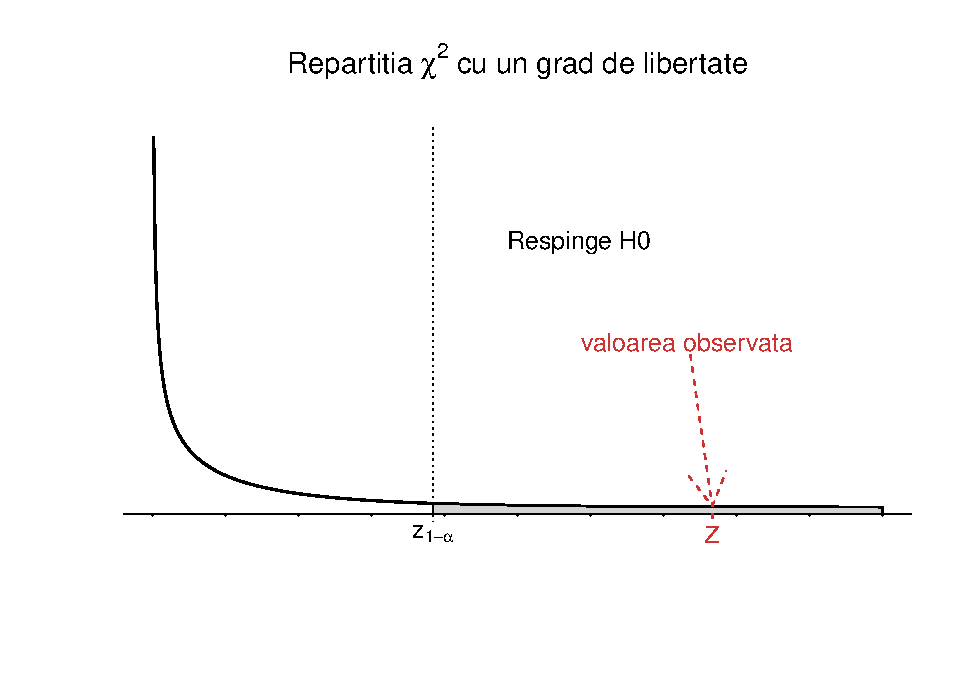
\includegraphics[width=0.8\linewidth]{Lab_5_files/figure-latex/unnamed-chunk-17-1} \end{center}

Același rezultat se obține și dacă folosim testul \texttt{prop.test},
acesta fiind un caz particular al testului hi-pătrat:

\begin{Shaded}
\begin{Highlighting}[]
\KeywordTok{prop.test}\NormalTok{(Mobs)}

    \DecValTok{2}\OperatorTok{-}\NormalTok{sample test }\ControlFlowTok{for}\NormalTok{ equality of proportions with continuity}
\NormalTok{    correction}

\NormalTok{data}\OperatorTok{:}\StringTok{  }\NormalTok{Mobs}
\NormalTok{X}\OperatorTok{-}\NormalTok{squared =}\StringTok{ }\FloatTok{7.6665}\NormalTok{, df =}\StringTok{ }\DecValTok{1}\NormalTok{, p}\OperatorTok{-}\NormalTok{value =}\StringTok{ }\FloatTok{0.005626}
\NormalTok{alternative hypothesis}\OperatorTok{:}\StringTok{ }\NormalTok{two.sided}
\DecValTok{95}\NormalTok{ percent confidence interval}\OperatorTok{:}
\StringTok{ }\FloatTok{0.0002463116} \FloatTok{0.0035536884}
\NormalTok{sample estimates}\OperatorTok{:}
\NormalTok{prop }\DecValTok{1}\NormalTok{ prop }\DecValTok{2} 
\FloatTok{0.0026} \FloatTok{0.0007} 
\end{Highlighting}
\end{Shaded}

\subsection{Metoda testului bazat pe raportul de
verosimilități}\label{metoda-testului-bazat-pe-raportul-de-verosimilitati}

În contextul exemplului de mai sus vrem să vedem testul bazat pe
raportul de verosimilitate. Considerând modelul multinomial
\((n_{11},n_{12},n_{21},n_{22})\sim \mathcal{M}(n;p_{11},p_{12},p_{21},p_{22})\),
obținem raportul de verosimilitate

\[
  \Lambda(x)=\frac{\sup_{\theta\in\Theta_0}L(\theta|x)}{\sup_{\theta\in\Theta}L(\theta|x)}=\prod_{i=1}^{2}\prod_{j=1}^{2}\left(\frac{n_{i\cdot}\times n_{\cdot j}}{n\times n_{ij}}\right)^{n_{ij}}
\]

și din teorema lui Wilks (cazul multidimensional) avem
\(-2\log\Lambda\to\chi^2(d-d_0)\) unde \(d=\dim(\Theta)\) și
\(d_0=\dim(\Theta_0)\). În cazul nostru

\[
  \begin{array}{ll}
    \Theta = \left\{(p_{11},p_{12},p_{21},p_{22})\,|\,p_{ij}\in(0,1),\,\sum_{i=1}^{2}\sum_{j=1}^{2}p_{ij}=1\right\}\\
    \Theta_0 = \left\{(p_{1}q_1,p_{1}q_2,p_{2}q_1,p_{2}q_2)\,|\,p_{i},q_j\in(0,1),\,\sum_{i=1}^{2}p_{i}=1,\,\sum_{j=1}^{2}q_j=1\right\}
  \end{array}
\]

unde \(p_i\) și \(q_j\) sunt repartițiile marginale. Obținem că
\(\dim(\Theta)=4-1\) iar \(\dim(\Theta_0)=4-2\), deci
\(-2\log\Lambda\to\chi^2(1)\).

\begin{Shaded}
\begin{Highlighting}[]
\CommentTok{# Observat}
\NormalTok{n11 =}\StringTok{ }\DecValTok{13}
\NormalTok{n1o =}\StringTok{ }\DecValTok{5000}
\NormalTok{n12 =}\StringTok{ }\NormalTok{n1o}\OperatorTok{-}\NormalTok{n11}

\NormalTok{n21 =}\StringTok{ }\DecValTok{7}
\NormalTok{n2o =}\StringTok{ }\DecValTok{10000}
\NormalTok{n22 =}\StringTok{ }\NormalTok{n2o}\OperatorTok{-}\NormalTok{n21}

\NormalTok{no1 =}\StringTok{ }\NormalTok{n11}\OperatorTok{+}\NormalTok{n21}
\NormalTok{no2 =}\StringTok{ }\NormalTok{n12}\OperatorTok{+}\NormalTok{n22}

\NormalTok{LRT =}\StringTok{ }\NormalTok{n11}\OperatorTok{*}\KeywordTok{log}\NormalTok{((n1o}\OperatorTok{*}\NormalTok{no1)}\OperatorTok{/}\NormalTok{(n}\OperatorTok{*}\NormalTok{n11)) }\OperatorTok{+}\StringTok{ }\NormalTok{n12}\OperatorTok{*}\KeywordTok{log}\NormalTok{((n1o}\OperatorTok{*}\NormalTok{no2)}\OperatorTok{/}\NormalTok{(n}\OperatorTok{*}\NormalTok{n12)) }\OperatorTok{+}\StringTok{ }
\StringTok{  }\NormalTok{n21}\OperatorTok{*}\KeywordTok{log}\NormalTok{((n2o}\OperatorTok{*}\NormalTok{no1)}\OperatorTok{/}\NormalTok{(n}\OperatorTok{*}\NormalTok{n21)) }\OperatorTok{+}\StringTok{ }\NormalTok{n22}\OperatorTok{*}\KeywordTok{log}\NormalTok{((n2o}\OperatorTok{*}\NormalTok{no2)}\OperatorTok{/}\NormalTok{(n}\OperatorTok{*}\NormalTok{n22))}
\NormalTok{LRT =}\StringTok{ }\OperatorTok{-}\DecValTok{2}\OperatorTok{*}\NormalTok{LRT}
\NormalTok{LRT}
\NormalTok{[}\DecValTok{1}\NormalTok{] }\FloatTok{8.354617}

\NormalTok{pval =}\StringTok{ }\DecValTok{1}\OperatorTok{-}\KeywordTok{pchisq}\NormalTok{(LRT,}\DecValTok{1}\NormalTok{) }\CommentTok{#df = 1}
\NormalTok{pval}
\NormalTok{[}\DecValTok{1}\NormalTok{] }\FloatTok{0.003847085}
\end{Highlighting}
\end{Shaded}

\begin{center}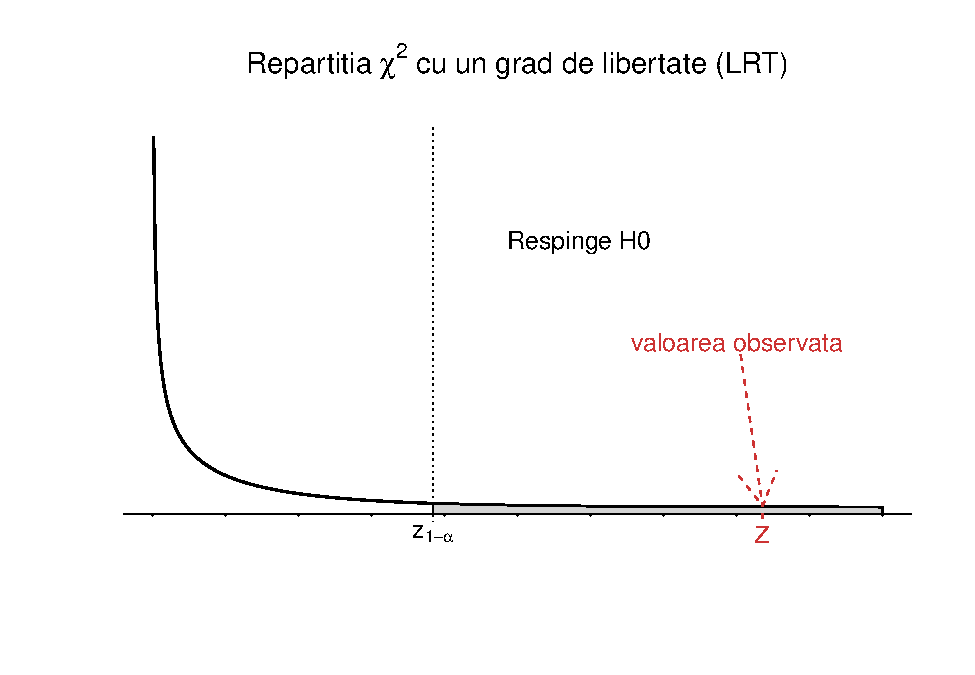
\includegraphics[width=0.8\linewidth]{Lab_5_files/figure-latex/unnamed-chunk-20-1} \end{center}

Să creăm o funcție care automatizează procesul:

\begin{Shaded}
\begin{Highlighting}[]
\NormalTok{LRT1 =}\StringTok{ }\ControlFlowTok{function}\NormalTok{(dat)\{}
  \CommentTok{# dat este sub forma de matrice }
\NormalTok{  rs =}\StringTok{ }\KeywordTok{rowSums}\NormalTok{(dat) }\CommentTok{# apply(dat, 1, sum)}
\NormalTok{  cs =}\StringTok{ }\KeywordTok{colSums}\NormalTok{(dat) }\CommentTok{# apply(dat, 2, sum)}
  
\NormalTok{  n =}\StringTok{ }\KeywordTok{sum}\NormalTok{(dat)}
  
\NormalTok{  expected <-}\StringTok{ }\KeywordTok{outer}\NormalTok{(rs,cs,}\StringTok{"*"}\NormalTok{)}\OperatorTok{/}\NormalTok{n}
  
\NormalTok{  lrt <-}\StringTok{ }\OperatorTok{-}\DecValTok{2}\OperatorTok{*}\KeywordTok{sum}\NormalTok{(dat }\OperatorTok{*}\StringTok{ }\KeywordTok{log}\NormalTok{(expected}\OperatorTok{/}\NormalTok{dat)) }
  
\NormalTok{  dm =}\StringTok{ }\KeywordTok{dim}\NormalTok{(dat) }\CommentTok{# dimensiunea tabloului pentru a calcula gradele de libertate}
\NormalTok{  pval =}\StringTok{ }\DecValTok{1}\OperatorTok{-}\KeywordTok{pchisq}\NormalTok{(lrt,(dm[}\DecValTok{1}\NormalTok{]}\OperatorTok{-}\DecValTok{1}\NormalTok{)}\OperatorTok{*}\NormalTok{(dm[}\DecValTok{2}\NormalTok{]}\OperatorTok{-}\DecValTok{1}\NormalTok{))}
  
  \KeywordTok{cat}\NormalTok{(}\StringTok{"Statistica LRT este "}\NormalTok{, lrt, }\StringTok{"}\CharTok{\textbackslash{}n}\StringTok{"}\NormalTok{)}
  \KeywordTok{cat}\NormalTok{(}\StringTok{"P-valoarea testului bazat pe raportul de verosimilitate este "}\NormalTok{, pval)}
  
  \KeywordTok{return}\NormalTok{(}\KeywordTok{list}\NormalTok{(}\DataTypeTok{statistic =}\NormalTok{ lrt, }\DataTypeTok{pvalue =}\NormalTok{ pval))}
\NormalTok{\}}

\NormalTok{Mobs =}\StringTok{ }\KeywordTok{matrix}\NormalTok{(}\KeywordTok{c}\NormalTok{(n11,n12,n21,n22),}\DataTypeTok{ncol =} \DecValTok{2}\NormalTok{, }\DataTypeTok{byrow =}\NormalTok{ T, }
              \DataTypeTok{dimnames =} \KeywordTok{list}\NormalTok{(}\KeywordTok{c}\NormalTok{(}\StringTok{"OC"}\NormalTok{,}\StringTok{"non-OC"}\NormalTok{), }\KeywordTok{c}\NormalTok{(}\StringTok{"MI"}\NormalTok{, }\StringTok{"non-MI"}\NormalTok{)))}

\KeywordTok{LRT1}\NormalTok{(Mobs) }
\NormalTok{Statistica LRT este  }\FloatTok{8.354617} 
\NormalTok{P}\OperatorTok{-}\NormalTok{valoarea testului bazat pe raportul de verosimilitate este  }\FloatTok{0.003847085}
\OperatorTok{$}\NormalTok{statistic}
\NormalTok{[}\DecValTok{1}\NormalTok{] }\FloatTok{8.354617}

\OperatorTok{$}\NormalTok{pvalue}
\NormalTok{[}\DecValTok{1}\NormalTok{] }\FloatTok{0.003847085}
\end{Highlighting}
\end{Shaded}

\section{Testul exact al lui Fisher}\label{testul-exact-al-lui-fisher}

\begin{rmdexercise}
Să presupunem că vrem să investigăm legătura dintre regimul bogat în
sare și decesul datorat unei boli cardiovasculare (CVD). Să presupunem
că suntem în contextul unui studiu retrospectiv efectuat pe un grup de
bărbați cu vârste cuprinse între 50 și 54 de ani dintr-o anumită regiune
geografică care au decedat pe parcursul unui luni. S-a încercat
introducerea în studiu a unui grup cât mai omogen (s-a încercat
includerea în studiu a unui număr egal de persoane care au decedat din
cauză de CVD și care au decedat din alte cauze).
\end{rmdexercise}

S-a obținut următorul tabel:

\rowcolors{2}{gray!6}{white}

\begin{longtable}{lccccccccc}
\hiderowcolors
\toprule
  & Ridicat Sare & Scazut Sare & Total\\
\midrule
\endfirsthead
\multicolumn{10}{@{}l}{\textit{(continued)}}\\
\toprule
  & Ridicat Sare & Scazut Sare & Total\\
\midrule
\endhead
\
\endfoot
\bottomrule
\endlastfoot
\showrowcolors
non-CVD & 2 & 23 & 25\\
CVD & 5 & 30 & 35\\
Total & 7 & 53 & 60\\*
\end{longtable}

\rowcolors{2}{white}{white}

Tabelul pe care ne așteptam să-l obținem (\(H_0\)) este:

\begin{Shaded}
\begin{Highlighting}[]
\CommentTok{# Observat}
\NormalTok{n11 =}\StringTok{ }\DecValTok{2}
\NormalTok{n1o =}\StringTok{ }\DecValTok{25}
\NormalTok{n12 =}\StringTok{ }\NormalTok{n1o}\OperatorTok{-}\NormalTok{n11}

\NormalTok{n21 =}\StringTok{ }\DecValTok{5}
\NormalTok{n2o =}\StringTok{ }\DecValTok{35}
\NormalTok{n22 =}\StringTok{ }\NormalTok{n2o}\OperatorTok{-}\NormalTok{n21}

\NormalTok{no1 =}\StringTok{ }\NormalTok{n11}\OperatorTok{+}\NormalTok{n21}
\NormalTok{no2 =}\StringTok{ }\NormalTok{n12}\OperatorTok{+}\NormalTok{n22}

\NormalTok{n =}\StringTok{ }\NormalTok{n1o}\OperatorTok{+}\NormalTok{n2o}

\CommentTok{#Asteptat}
\NormalTok{e11 =}\StringTok{ }\NormalTok{n1o}\OperatorTok{*}\NormalTok{no1}\OperatorTok{/}\NormalTok{n}
\NormalTok{e12 =}\StringTok{ }\NormalTok{n1o}\OperatorTok{*}\NormalTok{no2}\OperatorTok{/}\NormalTok{n}
\NormalTok{e21 =}\StringTok{ }\NormalTok{n2o}\OperatorTok{*}\NormalTok{no1}\OperatorTok{/}\NormalTok{n}
\NormalTok{e22 =}\StringTok{ }\NormalTok{n2o}\OperatorTok{*}\NormalTok{no2}\OperatorTok{/}\NormalTok{n}

\NormalTok{MobsF =}\StringTok{ }\KeywordTok{matrix}\NormalTok{(}\KeywordTok{c}\NormalTok{(n11,n12,n21,n22),}\DataTypeTok{ncol =} \DecValTok{2}\NormalTok{, }\DataTypeTok{byrow =}\NormalTok{ T, }
               \DataTypeTok{dimnames =} \KeywordTok{list}\NormalTok{(}\KeywordTok{c}\NormalTok{(}\StringTok{"non-CVD"}\NormalTok{, }\StringTok{"CVD"}\NormalTok{), }
                               \KeywordTok{c}\NormalTok{(}\StringTok{"Ridicat Sare"}\NormalTok{, }\StringTok{"Scazut Sare"}\NormalTok{)))}

\NormalTok{MexpF =}\StringTok{ }\KeywordTok{matrix}\NormalTok{(}\KeywordTok{c}\NormalTok{(e11,e12,e21,e22),}\DataTypeTok{ncol =} \DecValTok{2}\NormalTok{, }\DataTypeTok{byrow =}\NormalTok{ T, }
               \DataTypeTok{dimnames =} \KeywordTok{list}\NormalTok{(}\KeywordTok{c}\NormalTok{(}\StringTok{"non-CVD"}\NormalTok{, }\StringTok{"CVD"}\NormalTok{), }
                               \KeywordTok{c}\NormalTok{(}\StringTok{"Ridicat Sare"}\NormalTok{, }\StringTok{"Scazut Sare"}\NormalTok{)))}
\end{Highlighting}
\end{Shaded}

\rowcolors{2}{gray!6}{white}

\begin{longtable}{lcccccc}
\hiderowcolors
\toprule
  & Ridicat Sare & Scazut Sare\\
\midrule
\endfirsthead
\multicolumn{7}{@{}l}{\textit{(continued)}}\\
\toprule
  & Ridicat Sare & Scazut Sare\\
\midrule
\endhead
\
\endfoot
\bottomrule
\endlastfoot
\showrowcolors
non-CVD & 2.916667 & 22.08333\\
CVD & 4.083333 & 30.91667\\*
\end{longtable}

\rowcolors{2}{white}{white}

Observăm că avem două celule în tabelul așteptat care conțin mai puțin
de 5 observații prin urmare nu putem folosi metodele de mai sus
(aproximarea normală, testul lui Pearson sau testul bazat pe raportul de
verosimilitate). Dacă am încerca am obține:

\begin{Shaded}
\begin{Highlighting}[]
\CommentTok{# Testul lui Pearson (Hi patrat)}

\KeywordTok{chisq.test}\NormalTok{(MobsF)}

\NormalTok{    Pearson}\StringTok{'s Chi-squared test with Yates'}\NormalTok{ continuity correction}

\NormalTok{data}\OperatorTok{:}\StringTok{  }\NormalTok{MobsF}
\NormalTok{X}\OperatorTok{-}\NormalTok{squared =}\StringTok{ }\FloatTok{0.11552}\NormalTok{, df =}\StringTok{ }\DecValTok{1}\NormalTok{, p}\OperatorTok{-}\NormalTok{value =}\StringTok{ }\FloatTok{0.7339}

\CommentTok{# Testul bazat pe raportul de verosimilitate}

\KeywordTok{LRT1}\NormalTok{(MobsF)}
\NormalTok{Statistica LRT este  }\FloatTok{0.5810517} 
\NormalTok{P}\OperatorTok{-}\NormalTok{valoarea testului bazat pe raportul de verosimilitate este  }\FloatTok{0.4459004}
\OperatorTok{$}\NormalTok{statistic}
\NormalTok{[}\DecValTok{1}\NormalTok{] }\FloatTok{0.5810517}

\OperatorTok{$}\NormalTok{pvalue}
\NormalTok{[}\DecValTok{1}\NormalTok{] }\FloatTok{0.4459004}
\end{Highlighting}
\end{Shaded}

Enumerăm tabelele și probabilitățile lor de apariție:

\begin{Shaded}
\begin{Highlighting}[]
\CommentTok{# Fixez marginalele}

\NormalTok{n1o =}\StringTok{ }\DecValTok{25}
\NormalTok{n2o =}\StringTok{ }\DecValTok{35}
  
\NormalTok{no1 =}\StringTok{ }\DecValTok{7}
\NormalTok{no2 =}\StringTok{ }\DecValTok{53}

\ControlFlowTok{for}\NormalTok{ (i }\ControlFlowTok{in} \DecValTok{0}\OperatorTok{:}\DecValTok{7}\NormalTok{)\{}
  \KeywordTok{cat}\NormalTok{(}\StringTok{"-------------------------------------}\CharTok{\textbackslash{}n}\StringTok{"}\NormalTok{)}
  \KeywordTok{cat}\NormalTok{(}\StringTok{"Tabelul "}\NormalTok{, i}\OperatorTok{+}\DecValTok{1}\NormalTok{, }\StringTok{" :}\CharTok{\textbackslash{}n}\StringTok{"}\NormalTok{)}
  
  \CommentTok{# calculez valorile din tabel}
\NormalTok{  n11 =}\StringTok{ }\NormalTok{i}
\NormalTok{  n12 =}\StringTok{ }\NormalTok{n1o }\OperatorTok{-}\StringTok{ }\NormalTok{n11}
\NormalTok{  n21 =}\StringTok{ }\NormalTok{no1 }\OperatorTok{-}\StringTok{ }\NormalTok{n11}
\NormalTok{  n22 =}\StringTok{ }\NormalTok{no2 }\OperatorTok{-}\StringTok{ }\NormalTok{n12}
  
\NormalTok{  MobsF1 =}\StringTok{ }\KeywordTok{matrix}\NormalTok{(}\KeywordTok{c}\NormalTok{(n11,n12,n21,n22),}\DataTypeTok{ncol =} \DecValTok{2}\NormalTok{, }\DataTypeTok{byrow =}\NormalTok{ T, }
                  \DataTypeTok{dimnames =} \KeywordTok{list}\NormalTok{(}\KeywordTok{c}\NormalTok{(}\StringTok{"non-CVD"}\NormalTok{, }\StringTok{"CVD"}\NormalTok{), }
                                  \KeywordTok{c}\NormalTok{(}\StringTok{"Ridicat Sare"}\NormalTok{, }\StringTok{"Scazut Sare"}\NormalTok{)))}
  
  \KeywordTok{print}\NormalTok{(MobsF1)}
  
  \KeywordTok{cat}\NormalTok{(}\StringTok{"Probabilitatea de a obtine tabelul "}\NormalTok{, i}\OperatorTok{+}\DecValTok{1}\NormalTok{, }\StringTok{" este "}\NormalTok{, }
      \KeywordTok{dhyper}\NormalTok{(i, no1, no2, n1o), }\StringTok{"}\CharTok{\textbackslash{}n}\StringTok{"}\NormalTok{)}
  \KeywordTok{cat}\NormalTok{(}\StringTok{"-------------------------------------}\CharTok{\textbackslash{}n}\StringTok{"}\NormalTok{)}
\NormalTok{\}}
\OperatorTok{-------------------------------------}
\NormalTok{Tabelul  }\DecValTok{1}  \OperatorTok{:}
\StringTok{        }\NormalTok{Ridicat Sare Scazut Sare}
\NormalTok{non}\OperatorTok{-}\NormalTok{CVD            }\DecValTok{0}          \DecValTok{25}
\NormalTok{CVD                }\DecValTok{7}          \DecValTok{28}
\NormalTok{Probabilitatea de a obtine tabelul  }\DecValTok{1}\NormalTok{  este  }\FloatTok{0.0174117} 
\OperatorTok{-------------------------------------}
\OperatorTok{-------------------------------------}
\NormalTok{Tabelul  }\DecValTok{2}  \OperatorTok{:}
\StringTok{        }\NormalTok{Ridicat Sare Scazut Sare}
\NormalTok{non}\OperatorTok{-}\NormalTok{CVD            }\DecValTok{1}          \DecValTok{24}
\NormalTok{CVD                }\DecValTok{6}          \DecValTok{29}
\NormalTok{Probabilitatea de a obtine tabelul  }\DecValTok{2}\NormalTok{  este  }\FloatTok{0.1050706} 
\OperatorTok{-------------------------------------}
\OperatorTok{-------------------------------------}
\NormalTok{Tabelul  }\DecValTok{3}  \OperatorTok{:}
\StringTok{        }\NormalTok{Ridicat Sare Scazut Sare}
\NormalTok{non}\OperatorTok{-}\NormalTok{CVD            }\DecValTok{2}          \DecValTok{23}
\NormalTok{CVD                }\DecValTok{5}          \DecValTok{30}
\NormalTok{Probabilitatea de a obtine tabelul  }\DecValTok{3}\NormalTok{  este  }\FloatTok{0.2521695} 
\OperatorTok{-------------------------------------}
\OperatorTok{-------------------------------------}
\NormalTok{Tabelul  }\DecValTok{4}  \OperatorTok{:}
\StringTok{        }\NormalTok{Ridicat Sare Scazut Sare}
\NormalTok{non}\OperatorTok{-}\NormalTok{CVD            }\DecValTok{3}          \DecValTok{22}
\NormalTok{CVD                }\DecValTok{4}          \DecValTok{31}
\NormalTok{Probabilitatea de a obtine tabelul  }\DecValTok{4}\NormalTok{  este  }\FloatTok{0.3118225} 
\OperatorTok{-------------------------------------}
\OperatorTok{-------------------------------------}
\NormalTok{Tabelul  }\DecValTok{5}  \OperatorTok{:}
\StringTok{        }\NormalTok{Ridicat Sare Scazut Sare}
\NormalTok{non}\OperatorTok{-}\NormalTok{CVD            }\DecValTok{4}          \DecValTok{21}
\NormalTok{CVD                }\DecValTok{3}          \DecValTok{32}
\NormalTok{Probabilitatea de a obtine tabelul  }\DecValTok{5}\NormalTok{  este  }\FloatTok{0.214378} 
\OperatorTok{-------------------------------------}
\OperatorTok{-------------------------------------}
\NormalTok{Tabelul  }\DecValTok{6}  \OperatorTok{:}
\StringTok{        }\NormalTok{Ridicat Sare Scazut Sare}
\NormalTok{non}\OperatorTok{-}\NormalTok{CVD            }\DecValTok{5}          \DecValTok{20}
\NormalTok{CVD                }\DecValTok{2}          \DecValTok{33}
\NormalTok{Probabilitatea de a obtine tabelul  }\DecValTok{6}\NormalTok{  este  }\FloatTok{0.0818534} 
\OperatorTok{-------------------------------------}
\OperatorTok{-------------------------------------}
\NormalTok{Tabelul  }\DecValTok{7}  \OperatorTok{:}
\StringTok{        }\NormalTok{Ridicat Sare Scazut Sare}
\NormalTok{non}\OperatorTok{-}\NormalTok{CVD            }\DecValTok{6}          \DecValTok{19}
\NormalTok{CVD                }\DecValTok{1}          \DecValTok{34}
\NormalTok{Probabilitatea de a obtine tabelul  }\DecValTok{7}\NormalTok{  este  }\FloatTok{0.01604969} 
\OperatorTok{-------------------------------------}
\OperatorTok{-------------------------------------}
\NormalTok{Tabelul  }\DecValTok{8}  \OperatorTok{:}
\StringTok{        }\NormalTok{Ridicat Sare Scazut Sare}
\NormalTok{non}\OperatorTok{-}\NormalTok{CVD            }\DecValTok{7}          \DecValTok{18}
\NormalTok{CVD                }\DecValTok{0}          \DecValTok{35}
\NormalTok{Probabilitatea de a obtine tabelul  }\DecValTok{8}\NormalTok{  este  }\FloatTok{0.00124467} 
\OperatorTok{-------------------------------------}
\end{Highlighting}
\end{Shaded}

Aplicăm testul exact al lui Fisher \texttt{fisher.test}:

\begin{Shaded}
\begin{Highlighting}[]
\KeywordTok{fisher.test}\NormalTok{(MobsF)}

\NormalTok{    Fisher}\StringTok{'s Exact Test for Count Data}

\StringTok{data:  MobsF}
\StringTok{p-value = 0.6882}
\StringTok{alternative hypothesis: true odds ratio is not equal to 1}
\StringTok{95 percent confidence interval:}
\StringTok{ 0.04625243 3.58478157}
\StringTok{sample estimates:}
\StringTok{odds ratio }
\StringTok{  0.527113 }
\end{Highlighting}
\end{Shaded}

P-valoarea în \texttt{R} este calculată după formula:

\[
  p_{value} = \sum_{\{i:\mathbb{P}(i)\leq \mathbb{P}(obs)\}}\mathbb{P}(i)
\] care în cazul nostru devine

\begin{Shaded}
\begin{Highlighting}[]
\NormalTok{n1o =}\StringTok{ }\DecValTok{25}
\NormalTok{n2o =}\StringTok{ }\DecValTok{35}
  
\NormalTok{no1 =}\StringTok{ }\DecValTok{7}
\NormalTok{no2 =}\StringTok{ }\DecValTok{53}

\NormalTok{n11 =}\StringTok{ }\DecValTok{2}
  
\NormalTok{ps =}\StringTok{ }\KeywordTok{dhyper}\NormalTok{(}\DecValTok{0}\OperatorTok{:}\NormalTok{no1, no1, no2, n1o)}
\NormalTok{pobs =}\StringTok{ }\KeywordTok{dhyper}\NormalTok{(n11, no1, no2, n1o)}

\NormalTok{pval =}\StringTok{ }\KeywordTok{sum}\NormalTok{(ps[ps}\OperatorTok{<=}\NormalTok{pobs])}
\NormalTok{pval}
\NormalTok{[}\DecValTok{1}\NormalTok{] }\FloatTok{0.6881775}
\end{Highlighting}
\end{Shaded}

\section{Date pereche - Testul lui
McNemar}\label{date-pereche---testul-lui-mcnemar}

\begin{rmdexercise}
Ne propunem să comparăm două regimuri de chimioterapie pentru pacienții
cu cancer la sân care au efectuat operația de mastectomie. Cele două
grupuri de tratament investigate ar trebui să fie cât mai comparabile
din punct de vedere al celorlalți factori. Presupunem că un studiu de
potrivire (matched study) a fost pregătit așa încât din fiecare pereche
(potrivită din punct de vedere al vârstei și a condițiilor clinice) s-a
selectat aleator un membru căruia i-a fost administrat tratamentul A iar
celuilalt membru tratamentul B. Pacienții au fost urmăriți pe o perioadă
de 5 ani, iar variabila de interes a fost supraviețuirea în această
perioadă.
\end{rmdexercise}

S-au obținut următoarele date:

\rowcolors{2}{gray!6}{white}

\begin{longtable}{lccccccccc}
\hiderowcolors
\toprule
  & Supravietuit & Decedat & Total\\
\midrule
\endfirsthead
\multicolumn{10}{@{}l}{\textit{(continued)}}\\
\toprule
  & Supravietuit & Decedat & Total\\
\midrule
\endhead
\
\endfoot
\bottomrule
\endlastfoot
\showrowcolors
A & 526 & 95 & 621\\
B & 515 & 106 & 621\\
Total & 1041 & 201 & 1242\\*
\end{longtable}

\rowcolors{2}{white}{white}

Observăm că nu putem folosi testul lui Pearson (cu corecția lui Yates)
deoarece datele nu sunt \emph{independente}. Dacă am folosi am obține:

\begin{Shaded}
\begin{Highlighting}[]
\NormalTok{M1csq =}\StringTok{ }\KeywordTok{matrix}\NormalTok{(}\KeywordTok{c}\NormalTok{(}\DecValTok{526}\NormalTok{,}\DecValTok{95}\NormalTok{,}\DecValTok{515}\NormalTok{,}\DecValTok{106}\NormalTok{),}\DataTypeTok{ncol =} \DecValTok{2}\NormalTok{, }\DataTypeTok{byrow =}\NormalTok{ T)}
\KeywordTok{chisq.test}\NormalTok{(M1csq)}

\NormalTok{    Pearson}\StringTok{'s Chi-squared test with Yates'}\NormalTok{ continuity correction}

\NormalTok{data}\OperatorTok{:}\StringTok{  }\NormalTok{M1csq}
\NormalTok{X}\OperatorTok{-}\NormalTok{squared =}\StringTok{ }\FloatTok{0.59357}\NormalTok{, df =}\StringTok{ }\DecValTok{1}\NormalTok{, p}\OperatorTok{-}\NormalTok{value =}\StringTok{ }\FloatTok{0.441}
\end{Highlighting}
\end{Shaded}

Construim următorul tabel, în care unitatea de analiză nu mai este
\emph{pacientul} ci \emph{perechea} iar perechile sunt clasificate după
cum membrii acelei perechi au supraviețuit sau nu o perioadă
post-operatorie de 5 ani (liniile tabelului sunt rezultatele pacientului
care a urmat tratamentul A iar coloanele sunt rezultatele pacientului
care a urmat tratamentul B):

\rowcolors{2}{gray!6}{white}

\begin{longtable}{lccccccccc}
\hiderowcolors
\toprule
  & Supravietuit & Decedat & Total\\
\midrule
\endfirsthead
\multicolumn{10}{@{}l}{\textit{(continued)}}\\
\toprule
  & Supravietuit & Decedat & Total\\
\midrule
\endhead
\
\endfoot
\bottomrule
\endlastfoot
\showrowcolors
Supravietuit & 510 & 16 & 526\\
Decedat & 5 & 90 & 95\\
Total & 515 & 106 & 621\\*
\end{longtable}

\rowcolors{2}{white}{white}

Observăm că 600 (510+90) de perechi au avut același rezultat (perechi
concordante) și doar 21 de perechi au avut rezultate diferite (perechi
neconcordante).

Aplicăm testul lui McNemar \texttt{mcnemar.test} :

\begin{Shaded}
\begin{Highlighting}[]
\NormalTok{M1 =}\StringTok{ }\KeywordTok{matrix}\NormalTok{(}\KeywordTok{c}\NormalTok{(}\DecValTok{510}\NormalTok{,}\DecValTok{16}\NormalTok{,}\DecValTok{5}\NormalTok{,}\DecValTok{90}\NormalTok{),}\DataTypeTok{ncol =} \DecValTok{2}\NormalTok{, }\DataTypeTok{byrow =}\NormalTok{ T, }
           \DataTypeTok{dimnames =} \KeywordTok{list}\NormalTok{(}\KeywordTok{c}\NormalTok{(}\StringTok{"Supravietuit"}\NormalTok{, }\StringTok{"Decedat"}\NormalTok{), }
                           \KeywordTok{c}\NormalTok{(}\StringTok{"Supravietuit"}\NormalTok{, }\StringTok{"Decedat"}\NormalTok{)))}
\KeywordTok{mcnemar.test}\NormalTok{(M1)}

\NormalTok{    McNemar}\StringTok{'s Chi-squared test with continuity correction}

\StringTok{data:  M1}
\StringTok{McNemar'}\NormalTok{s chi}\OperatorTok{-}\NormalTok{squared =}\StringTok{ }\FloatTok{4.7619}\NormalTok{, df =}\StringTok{ }\DecValTok{1}\NormalTok{, p}\OperatorTok{-}\NormalTok{value =}\StringTok{ }\FloatTok{0.0291}
\end{Highlighting}
\end{Shaded}

\section{\texorpdfstring{Tabele de contingență
\(r\times c\)}{Tabele de contingență r\textbackslash{}times c}}\label{tabele-de-contingenta-rtimes-c}

\begin{rmdexercise}
Următorul tabel prezintă repartiția grupelor de sânge (A, B, AB și O) în
trei eșantioane de cetățeni afro-americani care trăiesc în trei state
diferite (Florida, Iowa și Missouri). Vrem să testăm la un nivel de
semnificație \(\alpha = 0.05\) dacă repartiția grupelor de sânge pentru
cetățenii afro-americani diferă de-a lungul celor trei state.
\end{rmdexercise}

\rowcolors{2}{gray!6}{white}

\begin{longtable}{lcccccccccccccccccccc}
\hiderowcolors
\toprule
  & A & B & AB & O & Total\\
\midrule
\endfirsthead
\multicolumn{21}{@{}l}{\textit{(continued)}}\\
\toprule
  & A & B & AB & O & Total\\
\midrule
\endhead
\
\endfoot
\bottomrule
\endlastfoot
\showrowcolors
Florida & 122 & 117 & 19 & 244 & 502\\
Iowa & 1781 & 1351 & 288 & 3301 & 6721\\
Missouri & 353 & 269 & 60 & 713 & 1395\\
Total & 2256 & 1737 & 367 & 4258 & 8618\\*
\end{longtable}

\rowcolors{2}{white}{white}

\subsection{\texorpdfstring{Testul \(\chi^2\) al lui
Pearson}{Testul \textbackslash{}chi\^{}2 al lui Pearson}}\label{testul-chi2-al-lui-pearson}

Tabelul pe care ne așteptăm să-l observat atunci când ipoteza nulă este
adevărată:

\begin{Shaded}
\begin{Highlighting}[]
\NormalTok{  matAA_observed =}\StringTok{ }\KeywordTok{rbind}\NormalTok{(}\KeywordTok{c}\NormalTok{(}\DecValTok{122}\NormalTok{, }\DecValTok{117}\NormalTok{, }\DecValTok{19}\NormalTok{, }\DecValTok{244}\NormalTok{),}
           \KeywordTok{c}\NormalTok{(}\DecValTok{1781}\NormalTok{, }\DecValTok{1351}\NormalTok{, }\DecValTok{288}\NormalTok{, }\DecValTok{3301}\NormalTok{),}
           \KeywordTok{c}\NormalTok{(}\DecValTok{353}\NormalTok{, }\DecValTok{269}\NormalTok{, }\DecValTok{60}\NormalTok{, }\DecValTok{713}\NormalTok{))}

\NormalTok{  rs =}\StringTok{ }\KeywordTok{rowSums}\NormalTok{(matAA_observed) }
\NormalTok{  cs =}\StringTok{ }\KeywordTok{colSums}\NormalTok{(matAA_observed) }
  
\NormalTok{  n =}\StringTok{ }\KeywordTok{sum}\NormalTok{(matAA_observed)}
  
\NormalTok{  matAA_expected <-}\StringTok{ }\KeywordTok{outer}\NormalTok{(rs,cs,}\StringTok{"*"}\NormalTok{)}\OperatorTok{/}\NormalTok{n}
\end{Highlighting}
\end{Shaded}

\rowcolors{2}{gray!6}{white}

\begin{longtable}{lcccccccccccccccccccc}
\hiderowcolors
\toprule
  & A & B & AB & O & Total\\
\midrule
\endfirsthead
\multicolumn{21}{@{}l}{\textit{(continued)}}\\
\toprule
  & A & B & AB & O & Total\\
\midrule
\endhead
\
\endfoot
\bottomrule
\endlastfoot
\showrowcolors
Florida & 131.4124 & 101.1806 & 21.37781 & 248.0292 & 502\\
Iowa & 1759.4078 & 1354.6504 & 286.21571 & 3320.7262 & 6721\\
Missouri & 365.1799 & 281.1691 & 59.40647 & 689.2446 & 1395\\
Total & 2256.0000 & 1737.0000 & 367.00000 & 4258.0000 & 8618\\*
\end{longtable}

\rowcolors{2}{white}{white}

Aplicând funcția \texttt{chisq.test} obținem:

\begin{Shaded}
\begin{Highlighting}[]
\KeywordTok{chisq.test}\NormalTok{(matAA_observed)}

\NormalTok{    Pearson}\StringTok{'s Chi-squared test}

\StringTok{data:  matAA_observed}
\StringTok{X-squared = 5.6382, df = 6, p-value = 0.4649}
\end{Highlighting}
\end{Shaded}

\subsection{Testul bazat pe raportul de
verosimilități}\label{testul-bazat-pe-raportul-de-verosimilitati}

Aplicând funcția \texttt{LRT1} construită anterior obținem p-valoarea
testului bazat pe raportul de verosimilitate:

\begin{Shaded}
\begin{Highlighting}[]
\KeywordTok{LRT1}\NormalTok{(matAA_observed)}
\NormalTok{Statistica LRT este  }\FloatTok{5.548169} 
\NormalTok{P}\OperatorTok{-}\NormalTok{valoarea testului bazat pe raportul de verosimilitate este  }\FloatTok{0.475654}
\OperatorTok{$}\NormalTok{statistic}
\NormalTok{[}\DecValTok{1}\NormalTok{] }\FloatTok{5.548169}

\OperatorTok{$}\NormalTok{pvalue}
\NormalTok{[}\DecValTok{1}\NormalTok{] }\FloatTok{0.475654}
\end{Highlighting}
\end{Shaded}

\subsection{Testul aproximat al lui
Fisher}\label{testul-aproximat-al-lui-fisher}

Testul exact al lui Fisher poate fi aplicat și în cazul tabelelor de tip
\(r\times c\) (pentru o generalizare a testului prezentat la curs puteți
consulta \url{http://mathworld.wolfram.com/FishersExactTest.html}) numai
că numărul de tabele pe care trebuie să le generăm devine prohibitiv. În
acest caz putem aproxima p-valoarea testului cu ajutorul metodelor de
tip Monte-Carlo. Mai multe informații despre testul lui Fisher (exact)
aproximat dar și despre alte teste exacte se găsesc în monografia (Mehta
and Patel 1995).

Generalizând raționamentul din cazul \(2 \times 2\) obținem că
probabilitatea (condiționată) de a observa un tabel dat fiind
marginalele (pe rânduri și pe coloane) este dată de:

\[
  \mathbb{P}(\,tabel\,) = \frac{\prod_{i=1}^{r}n_{i\cdot}!\prod_{j=1}^{c}n_{\cdot j}!}{n!\prod_{i=1}^{r}\prod_{j=1}^{c}n_{ij}!}\propto\frac{1}{\prod_{i=1}^{r}\prod_{j=1}^{c}n_{ij}!}
\] Pentru început să observăm că

\[
  \log(\mathbb{P}(\,tabel\,))\propto - \sum_{i=1}^{r}\sum_{j=1}^{c}\log(n_{ij}!) = - \sum_{i=1}^{r}\sum_{j=1}^{c}\log(\Gamma(n_{ij} + 1))
\]

iar pentru a calcula în R această probabilitate putem să folosim funcția
\texttt{lgamma()}. Ne punem acum întrebarea cum generăm aleator un tabel
cu \(r\) linii și \(c\) coloane care să aibă intrări numere naturale, a
căror sumă pe linii este \(n_{i\cdot}\) iar pe coloane este
\(n_{\cdot j}\).

O idee ar fi să ne uităm la indicii liniilor și a coloanelor (folosim
funcțiile \texttt{row()} și respectiv \texttt{col()}) și apoi să le
permutăm aleator (folosim \texttt{sample()}). Să presupunem că avem
tabelul \(2\times 2\)

\[
  \begin{array}{c|c|c|c}
     & 1 & 2 &\\
    \hline
    1 & n_{11} & n_{12} & n_{1\cdot}\\
    \hline
    2 & n_{21} & n_{22} & n_{2\cdot}\\
    \hline
     & n_{\cdot 1} & n_{\cdot 2} & n 
  \end{array}
\]

care mai poate fi scris, ținând seama doar de inidicii liniilor și
coloanelor pe care se află elementele, sub forma următoare

\[
  \underbrace{(1,1), (1,1), \ldots, (1,1)}_{n_{11}},\underbrace{(2,1), (2,1), \ldots, (2,1)}_{n_{21}},\underbrace{(1,2), (1,2), \ldots, (1,2)}_{n_{12}},\underbrace{(2,2), (2,2), \ldots, (2,2)}_{n_{22}}
\]

iar în R avem:

\begin{Shaded}
\begin{Highlighting}[]
\NormalTok{tab =}\StringTok{ }\KeywordTok{matrix}\NormalTok{(}\KeywordTok{c}\NormalTok{(}\DecValTok{10}\NormalTok{, }\DecValTok{3}\NormalTok{, }\DecValTok{5}\NormalTok{, }\DecValTok{7}\NormalTok{), }\DataTypeTok{nrow =} \DecValTok{2}\NormalTok{, }\DataTypeTok{byrow =} \OtherTok{TRUE}\NormalTok{)}
\NormalTok{tab}
\NormalTok{     [,}\DecValTok{1}\NormalTok{] [,}\DecValTok{2}\NormalTok{]}
\NormalTok{[}\DecValTok{1}\NormalTok{,]   }\DecValTok{10}    \DecValTok{3}
\NormalTok{[}\DecValTok{2}\NormalTok{,]    }\DecValTok{5}    \DecValTok{7}

\CommentTok{# liniile si coloanele pe care se afla elementele}
\KeywordTok{row}\NormalTok{(tab)}
\NormalTok{     [,}\DecValTok{1}\NormalTok{] [,}\DecValTok{2}\NormalTok{]}
\NormalTok{[}\DecValTok{1}\NormalTok{,]    }\DecValTok{1}    \DecValTok{1}
\NormalTok{[}\DecValTok{2}\NormalTok{,]    }\DecValTok{2}    \DecValTok{2}
\KeywordTok{col}\NormalTok{(tab)}
\NormalTok{     [,}\DecValTok{1}\NormalTok{] [,}\DecValTok{2}\NormalTok{]}
\NormalTok{[}\DecValTok{1}\NormalTok{,]    }\DecValTok{1}    \DecValTok{2}
\NormalTok{[}\DecValTok{2}\NormalTok{,]    }\DecValTok{1}    \DecValTok{2}

\CommentTok{# cream o lista cu doua componente}
\CommentTok{# prima corespunde indicilor liniilor}
\CommentTok{# a doua corespunde indicilor coloanelor}
\CommentTok{# cu nr de indici conform cu datele initiale}
\NormalTok{a =}\StringTok{ }\KeywordTok{list}\NormalTok{(}\KeywordTok{rep}\NormalTok{(}\KeywordTok{row}\NormalTok{(tab),tab), }\KeywordTok{rep}\NormalTok{(}\KeywordTok{col}\NormalTok{(tab),tab))}
\NormalTok{a}
\NormalTok{[[}\DecValTok{1}\NormalTok{]]}
\NormalTok{ [}\DecValTok{1}\NormalTok{] }\DecValTok{1} \DecValTok{1} \DecValTok{1} \DecValTok{1} \DecValTok{1} \DecValTok{1} \DecValTok{1} \DecValTok{1} \DecValTok{1} \DecValTok{1} \DecValTok{2} \DecValTok{2} \DecValTok{2} \DecValTok{2} \DecValTok{2} \DecValTok{1} \DecValTok{1} \DecValTok{1} \DecValTok{2} \DecValTok{2} \DecValTok{2} \DecValTok{2} \DecValTok{2} \DecValTok{2} \DecValTok{2}

\NormalTok{[[}\DecValTok{2}\NormalTok{]]}
\NormalTok{ [}\DecValTok{1}\NormalTok{] }\DecValTok{1} \DecValTok{1} \DecValTok{1} \DecValTok{1} \DecValTok{1} \DecValTok{1} \DecValTok{1} \DecValTok{1} \DecValTok{1} \DecValTok{1} \DecValTok{1} \DecValTok{1} \DecValTok{1} \DecValTok{1} \DecValTok{1} \DecValTok{2} \DecValTok{2} \DecValTok{2} \DecValTok{2} \DecValTok{2} \DecValTok{2} \DecValTok{2} \DecValTok{2} \DecValTok{2} \DecValTok{2}
\end{Highlighting}
\end{Shaded}

Vom afișa funcția care calculează p-valoarea testului lui Fisher prin
metoda Monte-Carlo:

\begin{Shaded}
\begin{Highlighting}[]
\NormalTok{fisher =}\StringTok{ }\ControlFlowTok{function}\NormalTok{(tab, }\DataTypeTok{n.sim=}\DecValTok{1000}\NormalTok{, }\DataTypeTok{return.all=}\OtherTok{FALSE}\NormalTok{, }\DataTypeTok{prnt=}\OtherTok{FALSE}\NormalTok{)\{}
\NormalTok{  bot0 =}\StringTok{ }\KeywordTok{sum}\NormalTok{(}\KeywordTok{lgamma}\NormalTok{(tab}\OperatorTok{+}\DecValTok{1}\NormalTok{))}\CommentTok{# lgamma: logaritm natural din gamma }
                            \CommentTok{#- logaritm din factorial}

\NormalTok{  bot =}\StringTok{ }\DecValTok{1}\OperatorTok{:}\NormalTok{n.sim}
\NormalTok{  a =}\StringTok{ }\KeywordTok{list}\NormalTok{(}\KeywordTok{rep}\NormalTok{(}\KeywordTok{row}\NormalTok{(tab),tab), }\KeywordTok{rep}\NormalTok{(}\KeywordTok{col}\NormalTok{(tab),tab))}
  
  \ControlFlowTok{for}\NormalTok{(i }\ControlFlowTok{in} \DecValTok{1}\OperatorTok{:}\NormalTok{n.sim) \{}
\NormalTok{    a[[}\DecValTok{1}\NormalTok{]] =}\StringTok{ }\KeywordTok{sample}\NormalTok{(a[[}\DecValTok{1}\NormalTok{]])}
\NormalTok{    bot[i] =}\StringTok{ }\KeywordTok{sum}\NormalTok{(}\KeywordTok{lgamma}\NormalTok{(}\KeywordTok{table}\NormalTok{(a)}\OperatorTok{+}\DecValTok{1}\NormalTok{))}
    \ControlFlowTok{if}\NormalTok{(prnt) \{ }\ControlFlowTok{if}\NormalTok{(i }\OperatorTok{==}\StringTok{ }\KeywordTok{round}\NormalTok{(i}\OperatorTok{/}\DecValTok{10}\NormalTok{)}\OperatorTok{*}\DecValTok{10}\NormalTok{) }\KeywordTok{cat}\NormalTok{(i,}\StringTok{"}\CharTok{\textbackslash{}n}\StringTok{"}\NormalTok{) \}}
\NormalTok{  \}}
  \ControlFlowTok{if}\NormalTok{(return.all) }\KeywordTok{return}\NormalTok{(}\KeywordTok{list}\NormalTok{(bot0, bot, }\KeywordTok{mean}\NormalTok{(bot0 }\OperatorTok{<=}\StringTok{ }\NormalTok{bot)))}
  \KeywordTok{cat}\NormalTok{(}\StringTok{"P-valoarea aproximata cu Monte Carlo este"}\NormalTok{, }\KeywordTok{mean}\NormalTok{(bot0 }\OperatorTok{<=}\StringTok{ }\NormalTok{bot))}
\NormalTok{\}}

\KeywordTok{set.seed}\NormalTok{(}\DecValTok{1234}\NormalTok{)}
\KeywordTok{fisher}\NormalTok{(matAA_observed)}
\NormalTok{P}\OperatorTok{-}\NormalTok{valoarea aproximata cu Monte Carlo este }\FloatTok{0.48}
\end{Highlighting}
\end{Shaded}

\begin{center}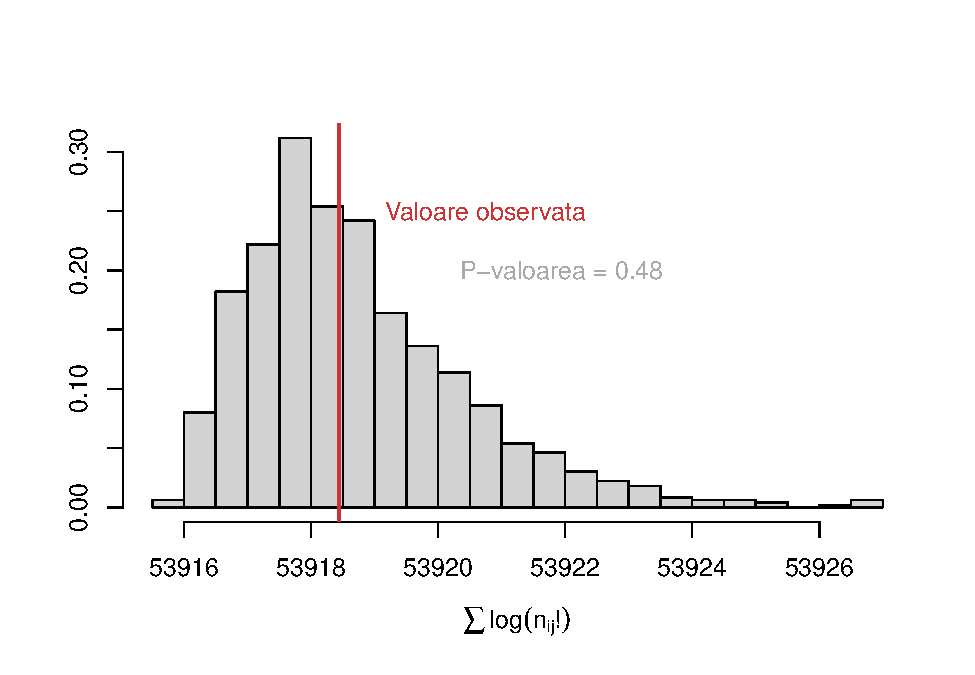
\includegraphics[width=0.8\linewidth]{Lab_5_files/figure-latex/unnamed-chunk-43-1} \end{center}

Același rezultat îl obținem și dacă folosim funcția
\texttt{fisher.test()} din R (care este mai rapidă):

\begin{Shaded}
\begin{Highlighting}[]
\KeywordTok{fisher.test}\NormalTok{(matAA_observed, }\DataTypeTok{simulate.p.value =} \OtherTok{TRUE}\NormalTok{, }\DataTypeTok{B =} \DecValTok{1000}\NormalTok{)}

\NormalTok{    Fisher}\StringTok{'s Exact Test for Count Data with simulated p-value (based}
\StringTok{    on 1000 replicates)}

\StringTok{data:  matAA_observed}
\StringTok{p-value = 0.4835}
\StringTok{alternative hypothesis: two.sided}
\end{Highlighting}
\end{Shaded}

\section*{Referințe}\label{referinte}
\addcontentsline{toc}{section}{Referințe}

\hypertarget{refs}{}
\hypertarget{ref-Agresti2000}{}
Agresti, Brian, Alan; Caffo. 2000. ``Simple and Effective Confidence
Intervals for Proportions and Differences of Proportions Result from
Adding Two Successes and Two Failures.'' \emph{The American
Statistician} 54: 280--88.
doi:\href{https://doi.org/10.1080/00031305.2000.10474560}{10.1080/00031305.2000.10474560}.

\hypertarget{ref-Mehta1995}{}
Mehta, Cyrus R., and Nitin R. Patel. 1995. \emph{Exact Tests}.
\url{http://gen.lib.rus.ec/book/index.php?md5=DDE1DF04691963EDA9F54E8942F48AA3}.


\end{document}
